% ============================================
% SECTION 4: METHODOLOGICAL FRAMEWORK
% How We Measure Cognitive Sovereignty
% ============================================
%
% FOCUS: The equation, R-values, measurement approaches
% 
% REMOVED (relocated):
% - Reconstruction possibilities → Section 7
% - Civilizational projections (2040-2050 window) → Section 8
% - Tainter threshold R < 0.05 → Section 8
% - Medieval university details → Section 6
%
% KEPT:
% - Core equation with SI units
% - R-value framework and table
% - Foundation-Specialization figure
% - Veterinarian contemporary proof
% ============================================

\section{Methodological Framework: Measuring Cognitive Sovereignty}
\label{sec:methodology}

This section presents the analytical tools for measuring cognitive sovereignty: the core thermodynamic equation, the R-value framework for quantifying extraction resistance, and validation through contemporary evidence.

\subsection{The Thermodynamic Equation}

Cognitive sovereignty can be expressed with physical simplicity:

\begin{equation}
\text{Cognitive Sovereignty [W]} = \frac{\text{Energy Invested [J]}}{\text{Time [s]}} \times \text{Resistance to Extraction [0-1]}
\label{eq:sovereignty}
\end{equation}

\noindent Where: Energy Investment Rate $>$ Entropy Rate

This formulation grounds abstract concepts in fundamental physics, using the same units (Watts) that \citet{smil2017} employs to trace energy transitions from agricultural societies ($10^4$ W/capita) through industrial ($10^5$ W/capita) to modern technological civilization ($10^6$ W/capita). Just as Smil demonstrates that civilizational complexity requires specific power densities, cognitive complexity requires specific power investments  above the brain's baseline consumption of approximately 20 Watts \citep{raichle2002}.

he equation's two multiplicative components yield precise diagnostic and predictive power:

\textbf{Power Component (J/s)}: Quantifies the rate of energy investment in cognitive development. This is measurable through time allocation: hours devoted to sustained learning, practice, and cross-domain synthesis.

\textbf{Resistance Component (R)}: Quantifies architectural quality---the degree to which cognitive structure resists algorithmic extraction. High-R architectures exhibit dense cross-domain connectivity, emergent synthesis capacity, and contextual adaptability. Low-R architectures exhibit linear specialization, procedural knowledge, and standardized outputs.

\subsection{The R-Value Framework}

To be unambiguous: R (extraction resistance) \textit{is} architectural quality, not a correlate or proxy. High-quality cognitive architecture manifests \textit{as} resistance to algorithmic extraction. Low-quality architecture manifests \textit{as} ease of proceduralization. The R-value doesn't measure something adjacent to quality; it operationally defines what quality means in thermodynamic terms.

Table~\ref{tab:r-values} presents the R-value framework with corresponding geometric, domain, and technological correlates:

\begin{table}[htbp]
\centering
\begin{tabular}{lllll}
\toprule
\textbf{R Range} & \textbf{Geometry} & \textbf{Cynefin Domain} & \textbf{Exemplar} & \textbf{AI Status} \\
\midrule
0.7--0.9 & Sphere & Chaotic & Renaissance polymath & Unreachable \\
0.4--0.7 & Ellipsoid & Complex & Complex navigator & GPT-5.x ceiling \\
0.2--0.4 & Cylinder & Complicated & Domain specialist & Current LLMs \\
0.0--0.2 & Vector & Clear & Procedural executor & Fully automated \\
\bottomrule
\end{tabular}
\caption{R-value framework mapping extraction resistance to cognitive geometry, Cynefin domains, and AI capability boundaries. Values represent theoretical positions based on documented characteristics, not empirical measurements.}
\label{tab:r-values}
\end{table}

These are theoretical positions based on documented characteristics, not empirical measurements. We \textit{define} a Renaissance polymath as exhibiting R $\approx$ 0.7--0.9 based on demonstrated capacity for cross-domain synthesis that resisted standardization for centuries. We \textit{position} current LLMs at R $\approx$ 0.1--0.2 based on observable performance in procedural versus emergent domains.

\subsection{Multiple Measurement Approaches}

We propose multiple measurement approaches, recognizing contextual specificity:

\begin{enumerate}
    \item \textbf{Dimensional Diversity ($R_1$)}: $R = 1 - (1/n)$, where $n$ represents integrated knowledge domains
    \item \textbf{Network Density ($R_2$)}: Ratio of actual to possible conceptual connections
    \item \textbf{Information Complexity ($R_3$)}: Kolmogorov incompressibility measure
    \item \textbf{Cynefin Classification ($R_4$)}: Domain-specific resistance \{Clear: 0.1, Complicated: 0.3, Complex: 0.7, Chaotic: 0.9\}
    \item \textbf{Knowledge Portfolio ($R_5$)}: Active knowledge types relative to historical maximum
\end{enumerate}

Practitioners may employ individual metrics or weighted combinations ($R = \sum w_i \times R_i$) appropriate to their specific context.

Critically, resistance exhibits temporal decay without maintenance:

\begin{equation}
R(t) = R_0 \times e^{-\lambda t}
\label{eq:decay}
\end{equation}

\noindent where $\lambda$ varies by knowledge type from 0.05/year for embodied skills to 1.0/year for micro-credentials. Skills unused decay; credentials unexercised become meaningless.

\subsection{Sphere Versus Vector: Architectural Definitions}

The geometric metaphor employed throughout this analysis represents measurable architectural differences:

\textbf{Sphere Architecture} represents multidimensional cognitive capacity:
\begin{itemize}
    \item Dense cross-domain connections enabling novel synthesis
    \item Multiple paths between concepts (network redundancy)
    \item Adaptive capacity across unfamiliar contexts
    \item Emergent insight from dimensional interaction
    \item High energy investment across many domains simultaneously
    \item Resistance to extraction through irreducible complexity
\end{itemize}

\textbf{Vector Architecture} represents unidimensional optimization:
\begin{itemize}
    \item Linear specialization along predetermined pathways
    \item Minimal cross-connections between knowledge domains
    \item Efficiency within bounded, familiar contexts
    \item Procedural responses to categorized inputs
    \item Low energy investment concentrated in single domain
    \item Vulnerability to extraction through complete documentability
\end{itemize}

These are not metaphors but observable properties. Network analysis can map conceptual connectivity. Performance metrics can assess adaptation versus optimization. Time allocation can quantify energy investment patterns. The sphere-to-vector transformation appears in observable changes: declining breadth of study, increasing specialization, reduced cross-domain practice.

\subsection{The Foundation-Specialization Ratio}

Historical analysis reveals a critical architectural metric: the proportion of educational investment devoted to comprehensive foundations versus specialized applications. Figure~\ref{fig:foundation-specialization} traces this ratio across 2,500 years.

\begin{figure}[htbp]
    \centering
    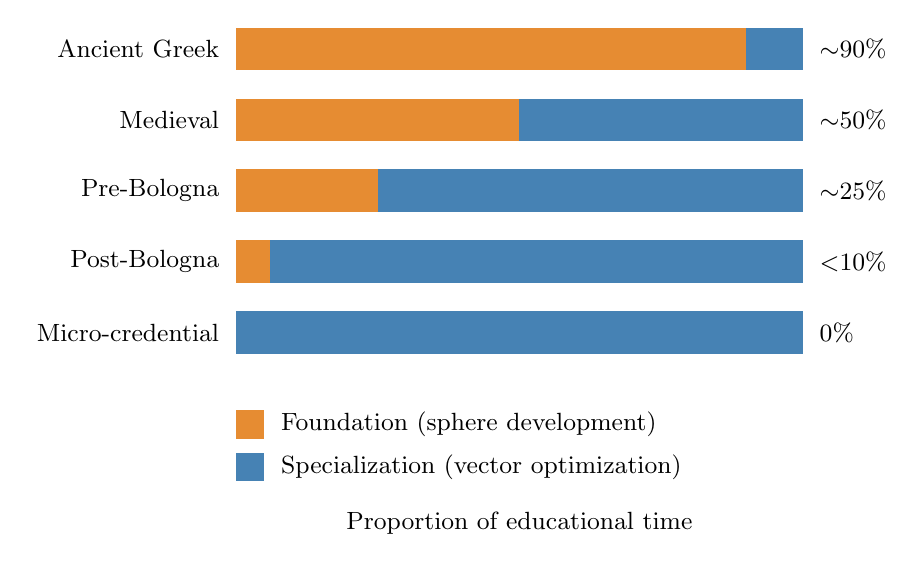
\begin{tikzpicture}[scale=0.9]
        % Define bar properties
        \def\barheight{0.6}
        \def\barwidth{8}
        \def\spacing{1.0}
        
        % Foundation color (orange/warm) and Specialization color (cold blue)
        \definecolor{foundation}{RGB}{230, 140, 50}
        \definecolor{specialization}{RGB}{70, 130, 180}
        
        % Ancient Greek: 90% foundation
        \fill[foundation] (0, 5*\spacing) rectangle (0.90*\barwidth, 5*\spacing+\barheight);
        \fill[specialization] (0.90*\barwidth, 5*\spacing) rectangle (\barwidth, 5*\spacing+\barheight);
        \node[left] at (-0.1, 5*\spacing+\barheight/2) {\small Ancient Greek};
        \node[right] at (\barwidth+0.1, 5*\spacing+\barheight/2) {\small $\sim$90\%};
        
        % Medieval: 50% foundation
        \fill[foundation] (0, 4*\spacing) rectangle (0.50*\barwidth, 4*\spacing+\barheight);
        \fill[specialization] (0.50*\barwidth, 4*\spacing) rectangle (\barwidth, 4*\spacing+\barheight);
        \node[left] at (-0.1, 4*\spacing+\barheight/2) {\small Medieval};
        \node[right] at (\barwidth+0.1, 4*\spacing+\barheight/2) {\small $\sim$50\%};
        
        % Pre-Bologna: 25% foundation
        \fill[foundation] (0, 3*\spacing) rectangle (0.25*\barwidth, 3*\spacing+\barheight);
        \fill[specialization] (0.25*\barwidth, 3*\spacing) rectangle (\barwidth, 3*\spacing+\barheight);
        \node[left] at (-0.1, 3*\spacing+\barheight/2) {\small Pre-Bologna};
        \node[right] at (\barwidth+0.1, 3*\spacing+\barheight/2) {\small $\sim$25\%};
        
        % Post-Bologna: <10% foundation
        \fill[foundation] (0, 2*\spacing) rectangle (0.06*\barwidth, 2*\spacing+\barheight);
        \fill[specialization] (0.06*\barwidth, 2*\spacing) rectangle (\barwidth, 2*\spacing+\barheight);
        \node[left] at (-0.1, 2*\spacing+\barheight/2) {\small Post-Bologna};
        \node[right] at (\barwidth+0.1, 2*\spacing+\barheight/2) {\small $<$10\%};
        
        % Micro-credential: 0% foundation
        \fill[specialization] (0, 1*\spacing) rectangle (\barwidth, 1*\spacing+\barheight);
        \node[left] at (-0.1, 1*\spacing+\barheight/2) {\small Micro-credential};
        \node[right] at (\barwidth+0.1, 1*\spacing+\barheight/2) {\small 0\%};
        
        % Legend - stacked vertically, left-aligned
        \fill[foundation] (0, -0.2) rectangle (0.4, 0.2);
        \node[right] at (0.5, 0) {\small Foundation (sphere development)};
        
        \fill[specialization] (0, -0.8) rectangle (0.4, -0.4);
        \node[right] at (0.5, -0.6) {\small Specialization (vector optimization)};
        
        % X-axis label
        \node at (4, -1.4) {\small Proportion of educational time};
    \end{tikzpicture}
    \caption{\textbf{The Foundation-Specialization Inversion (500 BCE--2025 CE).} Historical educational systems invested heavily in comprehensive foundations before permitting specialization. The architectural inversion correlates precisely with declining extraction resistance: orange warmth yields to blue cold as sphere collapses to vector.}
    \label{fig:foundation-specialization}
\end{figure}

The data reveal two simultaneous collapses:

\begin{enumerate}
    \item \textbf{Total energy reduction}: From 144 MJ (20 years $\times$ 2000 hours/year) to 0.144 MJ (40 hours)---a 1000-fold decrease
    \item \textbf{Foundation inversion}: From 90\% sphere-building to 0\%---complete architectural collapse
\end{enumerate}

The combination explains why modern credentials produce specialists vulnerable to AI replacement: they possess narrow vectors built on nonexistent spherical foundations.

\subsection{Contemporary Validation: The Veterinary Proof}

The framework gains validation through contemporary comparison of educational structures producing markedly different extraction resistance despite similar duration.

Human medicine and veterinary medicine both require approximately 8 years of post-secondary education. Yet their cognitive architectures differ fundamentally:

\textbf{Human Medicine (Specialist Vector)}:
\begin{itemize}
    \item Immediate specialization into organ systems
    \item Protocol-driven diagnostic pathways
    \item Single-species optimization
    \item Checklist-based clinical reasoning
    \item High vulnerability to AI diagnostic systems
\end{itemize}

\textbf{Veterinary Medicine (Generalist Sphere)}:
\begin{itemize}
    \item Comprehensive foundation across multiple species
    \item Pattern-recognition across biological diversity
    \item Continuous context-switching between anatomies
    \item Adaptive reasoning without species-specific protocols
    \item Significant resistance to algorithmic replacement
\end{itemize}

Lewis et al. (2022) document the ``scanning approach'' characteristic of veterinary clinical reasoning: broad initial assessment followed by contextual narrowing, contrasting with the linear algorithm application increasingly dominant in human medicine. Vandeweerd et al. (2013) confirm that veterinary expertise requires integration across ``widely different species and conditions,'' building cross-domain connectivity absent from single-species training.

The comparison provides controlled evidence: \textbf{same duration, different architecture, different R-values}. Time investment alone doesn't determine extraction resistance; architectural choices during that investment determine whether the result is sphere or vector.

As the saying among veterinarians goes: ``Real doctors treat more than one species.'' The joke contains thermodynamic truth.

\subsection{Methodological Limitations}

This framework operates at the level of structural analysis rather than individual prediction. We can identify architectural patterns that correlate with extraction resistance without claiming to measure any individual's precise R-value. The equation provides diagnostic and comparative tools, not personality assessment.

Additionally, R-values as presented are theoretical positions requiring empirical validation. The framework generates testable predictions---organizations with higher average R should show greater transformation success rates; individuals with more cross-domain training should demonstrate better novel-context performance---that future research can confirm or refute.

What the framework \textit{does} establish is the thermodynamic constraint: cognitive architectures require energy investment proportional to their complexity, and resistance to extraction correlates with that investment. These are physical relationships, not preferences. Section 5 examines why historical systems succeeded in making such investments while contemporary systems systematically fail.

% ============================================
% END SECTION 4
% ============================================
%
% FIGURE REQUIREMENTS:
% - figures/foundation-specialization.png (existing)
%
% CITATIONS USED:
% - Smil (2017)
% - Raichle & Gusnard (2002)
% - Lewis et al. (2022)
% - Vandeweerd et al. (2013)
%
% REMOVED CONTENT DESTINATIONS:
% - Reconstruction window 2040-2050 → Section 7/8
% - Tainter threshold R < 0.05 → Section 8
% - Civilizational cognitive power calculations → Section 8
% - Medieval curriculum details → Section 6
%
% HANDOFF TO SECTION 5:
% - "Why historical systems succeeded" question
% - Hidden energy budget framework
% ============================================